\documentclass[a4paper, 11pt, oneside]{book} % A4 paper size and default 11pt font size

\newcommand*{\plogo}{\fbox{$\mathcal{PL}$}} % Generic dummy publisher logo

%\usepackage[utf8]{inputenc} % Required for inputting international characters
%\usepackage[T1]{fontenc} % Output font encoding for international characters
%\usepackage{stix} % Use the STIX fonts

% 导入中文宏
\usepackage{ctex}
\usepackage{float}
\usepackage{indentfirst}
\usepackage{geometry}
\usepackage{amsmath}
\usepackage{setspace}
\usepackage{graphicx}
\numberwithin{equation}{subsection}
\usepackage{cite}
\usepackage{fancyhdr}
\usepackage{color}
\usepackage{appendix}
\usepackage{booktabs}  %table
\usepackage{listings} 
\usepackage{xcolor} 
\usepackage{fontspec}
\setmonofont{Consolas}

\geometry{left=2cm,right=2cm,top=2cm,bottom=2cm}
\setlength{\parindent}{2em}
	\vspace{10mm}

\lstset{
	backgroundcolor=\color{white},   % 选择代码背景,必须加上\ usepackage {color}或\ usepackage {xcolor}.
	basicstyle=\footnotesize,        % 设置代码字号.
	breakatwhitespace=false,         % 设置是否当且仅当在空白处自动中断.
	breaklines=true,                 % 设置自动断行.
	captionpos=b,                    % 设置标题位置.
	commentstyle=\color{green},    % 设置注释格式
	deletekeywords={...},            % 是否删除给定语言的关键词.
	escapeinside={\%*}{*)},          % 是否在代码中添加LaTex.
	extendedchars=true,              % 是否允许使用非ASCII字符; 仅适用于8位编码,不适用于UTF-8. 
	frame=single,	                   % 给代码区添加边框.
	keepspaces=true,                 % 保留空格(useful for keeping indentation of code (possibly needs columns=flexible).
	keywordstyle=\color{blue},       % 关键字显示风格.
	language=Octave,                 % 使用的语言.
	morekeywords={*,...},            % 是否需要添加其他的关键词.
	numbers=left,                    % 给代码添加行号,可取值none, left, right.
	numbersep=5pt,                   % 设置行号与代码之间的间隔
	numberstyle=\tiny\color{gray}, % 行号的字号和颜色
	rulecolor=\color{black},         % 边框颜色,如果没有设置,框架颜色可以在非黑色文本中的换行符上更改(例如 text (e.g. comments (green here)))
	showspaces=false,                % 显示每个地方添加特定下划线的空格; 覆盖了'showtringspaces'
	showstringspaces=false,          % 仅在字符串中允许空格
	showtabs=false,                  % show tabs within strings adding particular underscores
	stepnumber=2,                    % the step between two line-numbers. If it's 1, each line will be numbered
	stringstyle=\color{purple},     % string literal style
	tabsize=2,	                   % 将默认tab设置为2个空格
	title=\lstname                   % show the filename of files included with \lstinputlisting; also try caption instead of title
}


\pagestyle{fancy}
\lhead{}%左页眉
\chead{RISC-V on T-Core} %中间内容
\rhead{}  % 右边内容
\renewcommand\thesection{\arabic {section}}
\begin{document}
	\begin{titlepage} % Suppresses displaying the page number on the title page and the subsequent page counts as page 1
		
		\raggedleft % Right align the title page
		
		\rule{1pt}{\textheight} % Vertical line
		\hspace{0.05\textwidth} % Whitespace between the vertical line and title page text
		\parbox[b]{0.75\textwidth}{ % Paragraph box for holding the title page text, adjust the width to move the title page left or right on the page
			
			{\Huge\bfseries  课程实验报告}\\[2\baselineskip] % Title
			{\LARGE\textit{RISC-V on T-Core}}\\[4\baselineskip] % Subtitle or further description
			{\Large\textit{MaTrixV Team}} % Author name, lower case for consistent small caps
			
			\vspace{0.5\textheight} % Whitespace between the title block and the publisher
			
			{\noindent }\\[\baselineskip] % Publisher and logo
		}
	\end{titlepage}
	\tableofcontents
	\section{基础篇}
	\subsection{}
	\section{实践篇}
	
	\begin{figure}[H]
		\centering  
		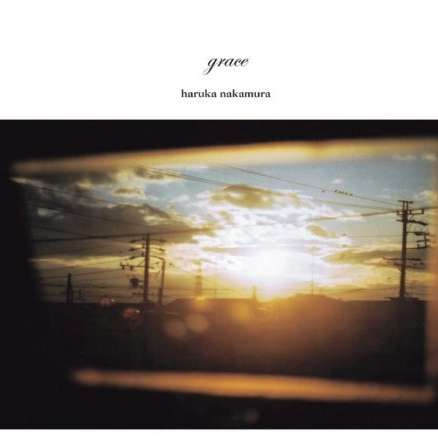
\includegraphics[scale=0.7]{img/avatar.jpg}   
		\caption{DHCP Request包字节形式}
	\end{figure}

	\begin{enumerate}
		\item 
	\end{enumerate}

	\begin{itemize}
		\item 
	\end{itemize}

	\begin{lstlisting}[language={C++}]
	class Pokemon : public QObject  	//代码
	\end{lstlisting}
	
	\begin{table}[H]
		\centering
		\begin{tabular}{lll}
			\hline
			字段 & 值 & 含义 \\ \hline
			包头长度 & 45 & 数据分组首部长度20字节 \\ \hline
			服务类型 & 00 & 正常时延、正常吞吐量、正常可靠性 \\ \hline
			总长度 & 003c & 数据分组长度60字节 \\ \hline
			标识 & 5c6e & 标识为23662 \\ \hline
			标志 & 00 & MF=0:此片为最后一片,DF=0:允许分片 \\ \hline
			片偏移 & 00 & 偏移量=0 \\ \hline
			TTL & 40 & 每跳生存周期为64 \\ \hline
			协议 & 01 & 来自ICMP协议 \\ \hline
			头部校验和 & 0000 & IP头部检验和为0000 \\ \hline
			源地址 & c0a86386 & 源地址为192.168.99.134 \\ \hline
			目的地址 & 72ff28a6 & 目的地址为114.255.40.166 \\ \hline
		\end{tabular}
	\end{table}
	
	\section{结果展示}
	
	\section{未来展望}
	
\end{document}